\documentclass[a4paper,11pt]{jarticle}
%\usepackage{graphicx}% Include figure files
\usepackage[dvipdfmx]{graphicx}
\usepackage{dcolumn}% Align table columns on decimal point
\usepackage{bm}% bold math
\usepackage{amssymb}
\usepackage{amsmath}

\def\vecR {\bm {\mathcal {R} } }
\def\R  {\mathcal {R} }
\pagestyle{plain}
\title{外場におけるダイポールを持った剛体}
\author{牧野真人}
\date{\number\year 年\number\month 月\number\day 日}
\begin{document}
\maketitle
%%%%%%%%%%%%
\section{理論}
図\ref{fig:system}のように、$x-y$平面に磁気ダイポール$\bm{p}=p\cos\theta\bm{e}_x+p\sin\theta\bm{e}_y$をもつ剛体を考える。
ここで$\theta$は$x$軸とダイポールがなす角度で時間の関数である。
$x-y$平面に垂直な軸のまわりの剛体の慣性モーメントは$I$とする。
一定磁場$\bm{B}=B\cos\alpha\bm{e}_x+B\sin\alpha\bm{e}_y$にあるとする。$\alpha$は$x$軸と磁場がなす角度である。
(べつに$x$軸と並行($\alpha=0$)でもいいんですけど)
たとえば、方位磁石が摩擦もない場合、北を向くがその場合の振動を考える。
\begin{figure}[h]
\centering
  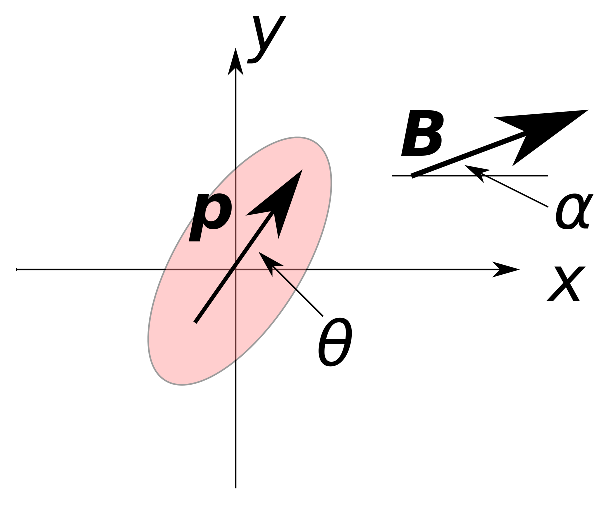
\includegraphics[clip,width=0.7\linewidth]{system.eps}
  \caption{一定磁場$\bm{B}$における磁気ダイポール$\bm{p}$を持った剛体。
  }
  \label{fig:system}
\end{figure}

回転の方程式は、
\begin{equation}
I\frac{d^2\theta}{dt^2}=p\cos\theta B\sin\alpha-p\sin\theta B\cos\alpha
\label{eq:basic}
\end{equation}
より、
\begin{equation}
\frac{d^2\theta}{dt^2}=-\omega^2\sin(\theta-\alpha)
\end{equation}
ここで、$\omega^2=pB/I$である。
この方程式の解は、
\begin{equation}
\theta=2\sin^{-1}k\mbox{sn}\left(\omega\left(t+\frac{T}{4}\right),k\right)+\alpha
\end{equation}
となる。snは楕円関数で、母数を
\begin{equation}
k^2=\sin^2\frac{\theta_0-\alpha}{2}
\end{equation}
とする。
ここで$\theta_0$は、初期の$\theta$の値で、このときは、$d\theta/dt=0$とする。
この議論は、単振り子の運動と同じである。
\section{シミュレーション}
\begin{verbatim}
dipole.udf
dipole_o.udf
\end{verbatim}
が入力、出力のudfである。
GOURMETより、
\begin{verbatim}
input_pendulums.py
\end{verbatim}
を使って入力udfの剛体の初期の角度$\theta_0$や磁場の角度$\alpha$などを変更できる。

\begin{verbatim}
output_angle.py
\end{verbatim}
をGOURMETより使って、時間と角度$\theta$を出力して、
\begin{verbatim}
plot_angle.py
\end{verbatim}
をgourmettermから、時間$t$と角度$\theta$および、解析解をプロット出来る。
図\ref{fig:time_angle}のとおりであり、シミュレーションと解析解が一致しているのが分かる。
\begin{figure}[h]
\centering
  \includegraphics[clip,width=0.9\linewidth]{time_angle.png}
  \caption{時間$t$に対する角度$\theta$。実線は解析解。
  }
  \label{fig:time_angle}
\end{figure}
\end{document}